\documentclass{article}
\usepackage{CJKutf8}
\usepackage{latexsym}
\usepackage{pgfplots}  
\usepackage{pgfplotstable}

\title{Week 10}
\author{软73 沈冠霖 2017013569}
\begin{document}
\begin{CJK}{UTF8}{gkai}
\maketitle
\section{T1}

\paragraph{算法}
对于P,先按照kmp算法的流程求出数组$\pi$。\\
之后先对于每个符号a,求出$\delta(0,a)$,有$\delta(0,a) = 1$当仅当P[1]=a,否则$\delta(0,a)=0$。\\
之后对于q=1 to m进行遍历,对于给定的q再对每个符号a进行遍历,如果$q \neq m \&\& P[q+1]=a$,则有$\delta(q,a)=q+1$,否则$\delta(q,a)=\delta(\pi[q],a)$。
\paragraph{复杂度}
根据kmp算法的结论,求出数组$\pi$的时间复杂度是$\theta(m)$。\\
求出$\delta(0,a)$的时间复杂度是$\theta(\Sigma)$。\\
而之后进行两层遍历,因为$\pi[q]<q$,因此在求$\delta(q,a)$的时候,$\delta(\pi[q],a)$必定已经求出来并且储存了,因此两层遍历中间的操作是$theta(1)$的,因此总共时间复杂度是$\theta(m\Sigma)$。
\paragraph{证明}
根据定义,$k=\delta(q,a)$等价于k为最大,满足$P_{i}\sqsupset P_{q}a$ 的i。因此,$t+1=\delta(q,a)$等价于t为最大的满足$P_{i}\sqsupset P_{q}$,且$P[i+1]=a$的i。\\
而根据kmp算法的结论,$P_{i}\sqsupset P_{q}$ 等价于$i \in \pi^{*}[q]\cup{q}$。此时,如果$P[i+1]=a \&\& i \neq m$,则q就是最大的i,$\delta(q,a)=q+1$。否则,只需要证明$\delta(\pi[q],a)-1$是最大的i即可。\\
首先证明$r = \delta(\pi[q],a)-1$是其中一个满足条件的i。因为$P_{r}\sqsupset P_{\pi[q]},P_{\pi[q]}\sqsupset P_{q}$,因此有$P_{r}\sqsupset P_{q}$,因此成立。\\
其次证明r是最大的i。假设有比r更大的i,令这个更大的为s,则如果$s \in \pi^{*}[q]$,则$P_{s}\sqsupset P_{\pi[q]},P[s+1]=a,s>r$,s就应该是$\delta(\pi[q],a)$,与$\delta(\pi[q],a) = r$矛盾。而如果s = q,则$P[s+1]=P[q+1] = a$,与$P[q+1] \neq a$或者$q=m$矛盾。因此r是最大的i,$\delta(q,a) = \delta(\pi[q],a)$。
\section{T2}
\subsection{1}
\paragraph{算法}
先按照kmp算法的流程求出$\pi$。\\
之后遍历i = 1 to m,令k = $i - \pi[i] > 0$,如果 $\pi[i] \neq 0$ 并且k = $\frac{\pi[i]}{\rho(P_{\pi_{i}})}$,则 $\rho(P_{\pi_{i}}) + 1$,否则$\rho(P_{i}) = 1$。\\
求$\pi$复杂度为$\theta(m)$,遍历的复杂度为$\theta(m)$,总共复杂度$\theta(m)$。
\paragraph{证明}
按照上述算法,$k = \rho(P_{i}) > 1$,等价于将集合$i\cup \pi^{*}[i]$从小到大排序,能构成公差为$\frac{i}{k}$的等差数列。只需要证明这个结论成立。\\
先证明充分性。如果$k = \rho(P_{i}) > 1$,则$P_{i}=w^{k}$,w为长度为$\frac{i}{k}$的串。只需要证明任意的$j = \pi^{t}[i]$,有$P_{j} = w^{k - t}$。用数学归纳法,在t = 0时,j = i,显然成立。而且,假设对于j = $\pi^{n}[i]$成立($j < k$),则$P_{j} = w^{k-j}$。$P_{j-|w|} = w^{k-j-1}\sqsupset P_{j}$成立。而如果能找到更大的$j - |v| > j - |w|$使得$\pi[j] = j - |v|$,则有对于任意的$ii \leq j - |v|,P[ii]=P[ii+|v|]$,而原本就有对于任意的$ii \leq j - |w|,P[ii]=P[ii+|w|]$,设tt为$|w|,|v|$的最大公约数,也有$P[ii]=P[ii+tt]$恒成立,则tt也可整除j,且商相比t更大,与$t = \rho(P_{j})$矛盾。充分性成立。\\
再证明必要性。如果能构成公差为$t = \frac{i}{k}$的等差数列,则对于任意的j,$\pi^{j+1}[i]=\pi^{j}[i] - t,\pi^{k}[i]=0,$,则有$w = P_{t}\sqsupset \forall P_{\pi^{j}[i]},j < k$,也就是$P_{\pi^{j+1}[i]}P_{t}=P_{\pi^{j}[i]},P_{i}=w^{k}$,必要性成立。\\
\subsection{2}
\paragraph{证明}
先给定串的长度m,字母表大小NUM,则最多有$NUM^{m}$个串。如果能证明对于给定的串长度,$E[\rho^{*}(P)] = O(1)$就可以证明结论成立。\\
$E[\rho^{*}(P)] = \frac{\sum_{i = 1}^{m} iNUM(i)}{NUM^{m}}$,其中NUM(i)为$\rho^{*}(P)=i$的长度为m的串个数。\\
如果$\rho^{*}(P)=i$,则必定能找到两个串w,v,使得$P = w^{i}v$,w有$NUM^{|w|}$种取值,v有$NUM^{|v|}$种取值,使得给定长度$|w|$,P最多有$NUM^{|w|+|v|}$种取值,而$i|w|\leq m$,使得$\rho^{*}(P)=i$的P最多有$\sum_{j=1}^{\frac{m}{i}}NUM^{m-j(i-1)}\leq NUM^{m+2-i}$。\\
这样,$\sum_{i = 1}^{m} iNUM(i)\leq \sum_{i=1}^{m}NUM^{m+2-i}i \leq 2NUM^{m+2}$,因此期望$E\leq 2NUM^{2} = O(1)$。
\subsection{3}
\paragraph{正确性}
如果模式串和待比较串的下一位相同,这个算法和kmp操作完全一致。否则,kmp算法是将两个串的相对位置向后移动了$q-\pi[[q]$位,而这个算法则是向后移动了$max(1,\lceil \frac{q}{\rho^{*}(P)+1}\rceil )$,则只需要证明这个数值恒小于等于$q-\pi[q]$即可。\\
首先,$1\leq q-\pi[q] $。其次,要证明$\lceil \frac{q}{\rho^{*}(P)+1}\rceil \leq q-\pi[q]$,只需要证明$q \leq (\rho^{*}(P)+1)(q-\pi[q])$。如果$q - \pi[q]$可以被q整除,那么根据上面的算法,有$\rho(P_{q})(q-\pi[q])=q$,式子成立。如果不可以被q整除,则有$P[i]=P[i+z(q-\pi[q])$对于任意的正整数z,在不超过范围的前提下成立。则必定可以找到最大的z使得$z(q-\pi[q])\leq P_{q}$,有$P_{z(q-\pi[q])}=w^{z}$,且$q\leq(z+1)(q-\pi[q])$,此时有$z\leq \rho^{*}(P)$,因此有$q \leq (\rho^{*}(P)+1)(q-\pi[q])$。
\paragraph{复杂度}
求$\rho^{*}(P)$的复杂度是$\theta(m)$。而在第i轮while循环中,s增加了$\lceil\frac{q_{i}}{k}\rceil$,而q增加了$O(q_{i})$次。假设t轮跳出循环,则此时$\sum_{i=1}^{t}\lceil\frac{q_{i}}{k}\rceil = O(n),\sum_{i=1}^{t}O(q_{i}) =O(kn)$。因此有总共复杂度为$O(m+\rho^{*}(P)n)$
\section{T3} 
\paragraph{测试环境}
CPU:Inter Core i5-6300HQ,2.3GHZ\\
内存:12G\\
环境:VS2017,release模式
\paragraph{算法原理}
几种字符串匹配算法的原理和课上讲的完全一致。只额外提到一点:
我的RabinKarp算法没有做取余运算,因为int类型数据的加法和乘法在溢出后会自动取余。
\paragraph{结果正确性}
无论是用课上的数据验证,还是自己设计数据,还是随机生成数据,五种算法得到的结果都完全一致,可以说明算法正确。
\subsection{运行时间分析}
具体的运行时间结果见下表1,2和折线图1,2。\\
\paragraph{固定模式串长度m,测试不同待比较字符串长度n的运行时间}
首先,每个算法的运行时间大致都是线性增长的,和他们理论上对n的线性复杂度相符。\\
其次,这几种算法中,Rabin-Karp算法最慢,其次是有限自动机算法,KMP算法和Boyer-Moore算法差不多,最快的是Naive算法。我猜想原因如下:\\
1.因为模式串很短,只有5,而且是随机生成的,因此出现重复模式的概率很低,因此利用自相似性的有限自动机算法和KMP算法效率都很低,而有限自动机算法每次都访问一个二维数组,而且需要把字符转码成为数字才能访问,因此效率更低。\\
2.因为我用了一共72个字符,数值计算本身就很耗费时间,因此Rabin-Karp的常数k很大,效率非常低下。\\
3.因为模式串自相似性很低,因此Boyer-Moore算法每次能够跳过几乎整个模式串的长度,但是模式串长度本身就低,因此其效果也没那么好。\\
\paragraph{固定待比较字符串长度长度n,测试不同模式串长度m的运行时间}
首先,随着m的增长,除了Boyer-Moore之外,每个算法运行时间大概不变。对于后三个算法这比较好理解,因为n远大于m,而他们运行时间都是$\theta(n)$,而初始化时间相对运行时间可以忽略不计,因此他们运行时间大概不变。而这和Naive算法$O(mn)$的复杂度差别很大,可能是体系结构层次的问题了。\\
而对于Boyer-Moore来说,因为模式串是随机生成的,自相似性很低,因此每次几乎能跳过大半个乃至整个模式串,因此复杂度应该是近似其最好情况的复杂度$O(\frac{n}{m})$的,因此随着m的增加,运行时间在减少。\\
其次,除了Boyer-Moore算法之外,另外四个算法的时间仍然是Naive快于KMP快于有限自动机快于Rabin-Karp,我猜想原因与之前的分析一致。\\
而在模式串长度较短的情况下,Boyer-Moore算法的确不是很好,但是模式串长度较长的时候,这个算法是最快的。我猜想其原因仍旧同上。而想必这也是在文本编辑器中多使用这个算法的原因了,因为一篇文章里要查询的词,句子等自相似性不会很高,而且其长度一般大于等于10。这种情况下Boyer-Moore的运行时间不亚于甚至高于其他算法。\\
\begin{table}[!htbp] 
	
	\caption{待比较字符串为不同长度时各个算法运行时间}
	\begin{flushleft} 
		
		\begin{tabular}{|l|l|l|l|l|l|l|l|l|l|l|} 
			\hline 测量序号 & 1 & 2 & 3 & 4 & 5 & 6 & 7 & 8\\ 
			\hline 待比较串长度 &10&100&1000&10000&100000&1000000&10000000&100000000 \\ 
			\hline Naive算法执行时间 (ms)
			&0&0&0&0&0.2&1.4&13.2&127.4  \\
			\hline Rabin-Karp算法执行时间 (ms)
			&0&0&0.2&0.4&1.8&19.6&196&1970.4  \\ 
			\hline DFA算法执行时间 (ms)
			&0&0&0&0&1&11.2&109.4&1083.4  \\ 
			\hline KMP算法执行时间 (ms)
			&0&0&0&0.2&0.2&2.8&27.8&278.2  \\ 
			\hline Boyer-Moore算法执行时间 (ms)
			&0&0&0&0&0.6&3&29&292.2  \\ 
			\hline 
		\end{tabular} 
		注:每组数据都是运行5次后取的平均值,模式串长度均为5\\
	\end{flushleft} 
\end{table}
\begin{table}[!htbp] 
	
	\caption{模式串为不同长度时各个算法运行时间}
	\begin{flushleft} 
		
		\begin{tabular}{|l|l|l|l|l|l|l|l|l|l|l|} 
			\hline 测量序号 & 1 & 2 & 3 & 4 & 5 & 6 & 7 & 8\\ 
			\hline 模式串长度 &2&5&10&20&50&100&300&1000 \\ 
			\hline Naive算法执行时间 (ms)
			&13&12.4&12.2&13&13&12.4&12.2&12.4  \\
			\hline Rabin-Karp算法执行时间 (ms)
			&156&194.6&194.4&192.8&194.8&193.4&193.8&192.4  \\ 
			\hline DFA算法执行时间 (ms)
			&106.4&107.4&108.6&106&106.6&108.6&107&105.4  \\ 
			\hline KMP算法执行时间 (ms)
			&28&27.2&28&28&27.2&28.2&27.8&27.2  \\ 
			\hline Boyer-Moore算法执行时间 (ms)
			&69.8&28.8&14.6&8.2&4.2&3.6&2.8&2.8  \\ 
			\hline 
		\end{tabular} 
		注:每组数据都是运行5次后取的平均值,待比较串长度均为10000000\\
	\end{flushleft} 
\end{table}


\pgfplotsset{}

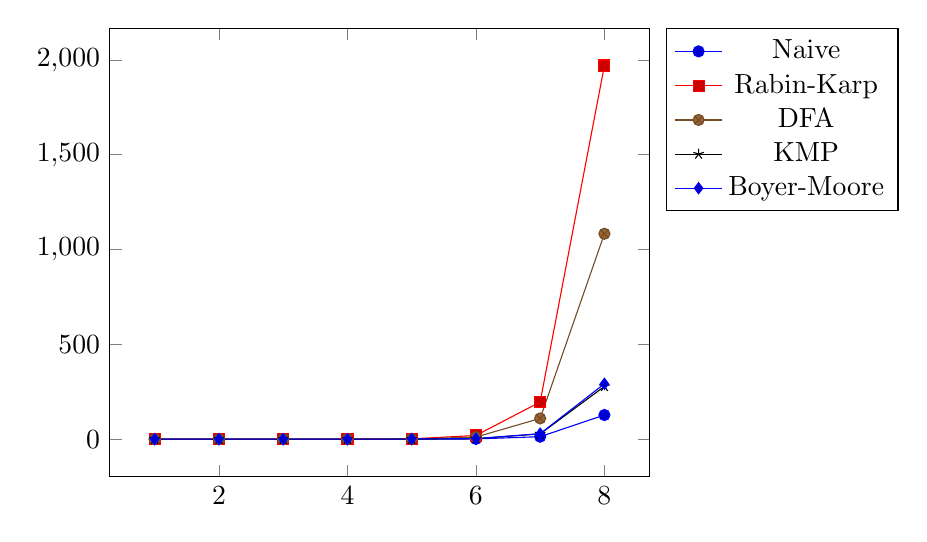
\begin{tikzpicture}

\begin{axis}[legend pos=outer north east] % 将图例放在图外,位于图的东北角
\addplot 
table[]                         
{           		                
	N T
	1 0
	2 0
	3 0
	4 0 
	5 0.2
	6 1.4
	7 13.2
	8 127.4
};
\addplot 
table[]                         
{           		                
	N T
	1 0
	2 0
	3 0.2
	4 0.4 
	5 1.8
	6 19.6
	7 196
	8 1970.4
};
\addplot 
table[]                         
{           		                
	N T
	1 0
	2 0
	3 0
	4 0 
	5 1
	6 11.2
	7 109.4
	8 1083.4
};

\addplot 
table[]                         
{           		                
	N T
	1 0
	2 0
	3 0
	4 0.2
	5 0.2
	6 2.8
	7 27.8
	8 278.2
};

\addplot 
table[]                         
{           		                
	N T
	1 0
	2 0
	3 0
	4 0 
	5 0.6
	6 3
	7 29
	8 292.2
};
\addlegendentry{Naive}         
\addlegendentry{Rabin-Karp}
\addlegendentry{DFA}
\addlegendentry{KMP}
\addlegendentry{Boyer-Moore}
\end{axis}

\end{tikzpicture}



\pgfplotsset{}

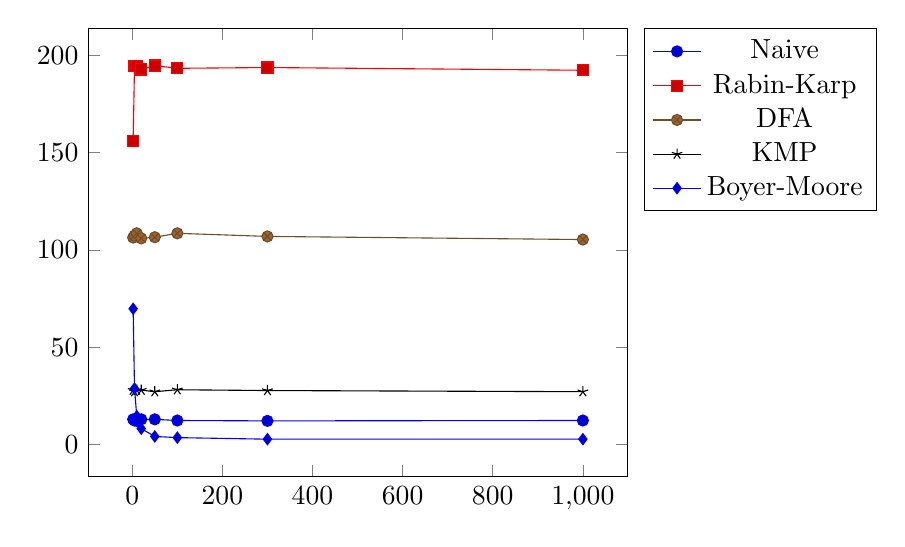
\begin{tikzpicture}

\begin{axis}[legend pos=outer north east] % 将图例放在图外,位于图的东北角
\addplot 
table[]                         
{           		                
	N T
	2 13
	5 12.4
	10 12.2
	20 13 
	50 13
	100 12.4
	300 12.2
	1000 12.4
};

\addplot 
table[]                         
{           		                
	N T
	2 156
	5 194.6
	10 194.4
	20 192.8
	50 194.8
	100 193.4
	300 193.8
	1000 192.4
};

\addplot 
table[]                         
{           		                
	N T
	2 106.4
	5 107.4
	10 108.6
	20 106
	50 106.6
	100 108.6
	300 107
	1000 105.4
};

\addplot 
table[]                         
{           		                
	N T
	2 28
	5 27.2
	10 28
	20 28
	50 27.2
	100 28.2
	300 27.8
	1000 27.2
};

\addplot 
table[]                         
{           		                
	N T
	2 69.8
	5 28.8
	10 14.6
	20 8.2
	50 4.2
	100 3.6
	300 2.8
	1000 2.8
};
\addlegendentry{Naive}         
\addlegendentry{Rabin-Karp}
\addlegendentry{DFA}
\addlegendentry{KMP}
\addlegendentry{Boyer-Moore}
\end{axis}

\end{tikzpicture}



\end{CJK}
\end{document}
